\documentclass[titlepage]{article}
\usepackage{graphicx}
\usepackage[tbtags]{amsmath}

\begin{document}

\title{Experiment 3: Conservation of Mechanical Energy}
\author{Tian Ye \\ \\ UID: 704931660 \\ \\ TA: Wen Li Wen \\ \\ Lab Partner: Chris Ong \\ \\ Lab 8 Tuesday 6:00 PM}
\date{October 24th, 2017}

\maketitle

\vspace*{\fill}
\begin{center}
\section*{Conservation of Energy in a Simple Harmonic Oscillator}
T. Ye\textsuperscript{1}
\hfill
\begin{minipage}{1\textwidth}
\hfill \\
\hfill \\
In Classical Physics, mechanical energy is said to be conserved per the law of Conservation of Energy. To test this principle, a glider with a photocomb attached to the top of it was set into simple harmonic oscillation via a spring system. A photogate recorded the time intervals at which each tooth in the comb passed it while the glider was moving in half a complete oscillation. To calculate the spring constant in order to solve for spring potential energy, the displacement of the glider relative to force applied was recorded and plotted - the slope of said relation equating the spring constant. To calculate kinetic energy of the glider, the displacement of the glider was differentiated with respect to time in order to solve for velocity. A plot describing the relations between spring potential energy, kinetic energy of the glider, and total mechanical energy of the system was then created. From the plot it can be seen that total mechanical energy decreases only very slightly, which is to be expected as no system is completely frictionless, resulting in some non-conserved work due to friction. Therefore the system demonstrates the law of Conservation of Energy.
\hfill \\

\footnotesize{\textsuperscript{1}Henry Samueli School of Engineering and Applied Sciences, Univ. California Los Angeles}

\hfill \\

\scriptsize{Word Count: 195}
\end{minipage}
\end{center}
\vfill

\pagebreak

\section{Introduction}
The premise of Experiment 3 is to measure the total mechanical energy of a spring-glider system and the energy that it loses to kinetic friction while oscillating. This is accomplished via setting a glider with a comb attached on top of it into oscillation while a photogate measures the elapsed time interval between every comb tooth that passes it. A diagram of the setup is shown below:

\begin{figure}[!htbp]
    \centering
    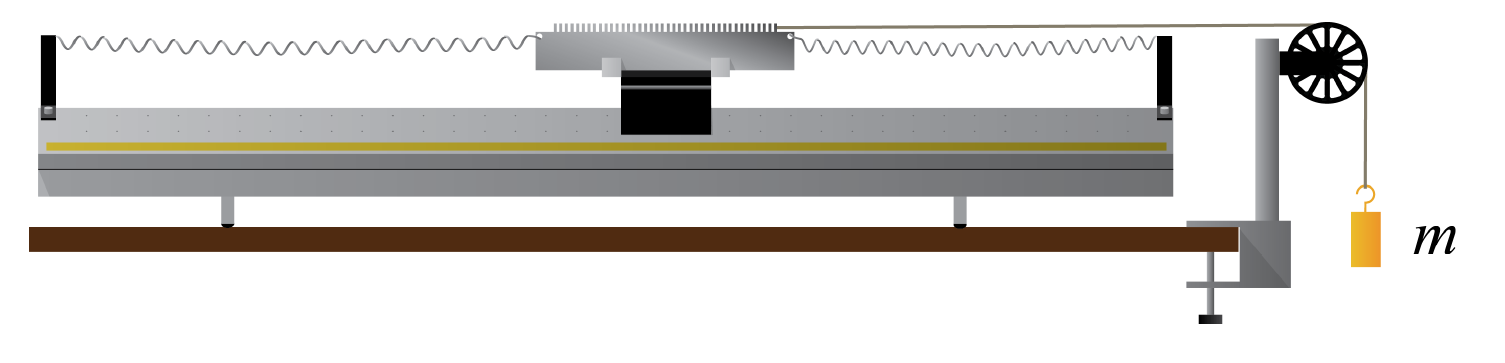
\includegraphics[width=5.0in]{Setup.png}
    \caption{Visual representation of the glider, comb, spring, and photogate system. Note: the hanging mass and pulley were only used to calculate $k$, the spring constant, and were removed for the actual oscillation tests. Figure reproduced (with permission) from Fig. 3.1 by Campbell, W. C. \textit{et al.\textsuperscript{1}}.}
\end{figure}

\section{Calculations}
For any given oscillation, we know that the total mechanical energy can be expressed as following:

\begin{align}
E\textsubscript{total} = K + U
\end{align}

\begin{center}
Where $K = \frac{1}{2}mv^2$ and $U = \frac{1}{2}kx^2$.
\end{center}

\subsection{Solving for $K$}
In order to find $K$, we must first solve for velocity of the glider. Using the expression $\Delta v = \frac{\Delta x}{\Delta t}$, we find that we must solve for the displacement. Using the fact that each gap of the comb is 2 mm wide and each ``tooth" of the comb is 2 mm wide, we can set $\lambda$, the distance that the comb has travelled between each timestamp, as 4 mm.

From this we can then use the equation $v(x) = \frac{x\textsubscript{i+1}-x_i}{t\textsubscript{i+1}-t_1}$, with the value of the numerator always being 4 mm, as the displacement between two teeth will always be 4 mm. Using the value of the calculated average velocity, we can then find $K$ by plugging $v$ into $K = \frac{1}{2}mv^2$, with mass being the mass of the glider and comb: $m = (225 \pm 1)$ g.

\subsection{Solving for $U$}
In order to solve for $U$, we cannot directly use the equation $U = \frac{1}{2}kx^2$, as the velocity calculated previously was average velocity between each time interval. Consequently, for the spring potential energy, we must use average displacement between each time interval as well. To solve for the average displacement per time interval, we use the equation $\bar x = \frac{1}{2}(x\textsubscript{i+1}+x_i)$. When we conducted the experiment, we placed the photogate so that at equilibruim, it was positioned on the 31st tooth. Given that there are 61 teeth total and that $\lambda$ is 4 mm, we can state the displacement at any given point as $x_n = 0.004(n - 31)$, where n refers to the data point corresponding to the nth tooth in the comb. Therefore, the recorded amplitude of displacement is $\pm$ 0.118 meters.

\subsubsection{Solving for $k$}
Referring back to Figure 1 in the introduction, we solved for $k$ by hanging a mass over a pulley and waiting for the system to reach a new equilibruim. By measuring the displacement of the glider from the original equilibrium, we could solve for the spring constant $k$ as the force of gravity on the mass, $mg$, is equal to the tension force of the string which is equal to the spring force.

\begin{table}[!htbp]
\renewcommand{\arraystretch}{1.3}
\centering
\begin{tabular}{c|c|c}
    \hline
    \hline
    Mass (grams) & Force (N) & Displacement (m)\\
    \hline
    \hline

    3.5 $\pm$ 0.5    &  0.034 &  0.005 $\pm$ 0.5\\
    \hline

    5.0 $\pm$ 0.5    &  0.049 &  0.006 $\pm$ 0.5\\
    \hline

    19.5 $\pm$ 0.5   &  0.191 &  0.030 $\pm$ 1.0\\
    \hline

    36.0 $\pm$ 0.5   &  0.353 &  0.059 $\pm$ 0.5\\
    \hline

    55.5 $\pm$ 1.0  &  0.544 &  0.093 $\pm$ 0.5\\
    \hline
\end{tabular}
\caption{Recorded data used to solve for $k$. Leftmost column represents the measured mass of the hanging masses, center column represents calculated force using 9.8 m/s$^2$ for $g$, and rightmost column represents measured displacement from equilibrium.}
\end{table}

Plotting the calculated force against the measured displacement, we are presented with the following plot on the next page:

\pagebreak

\begin{figure}[!htbp]
    \centering
    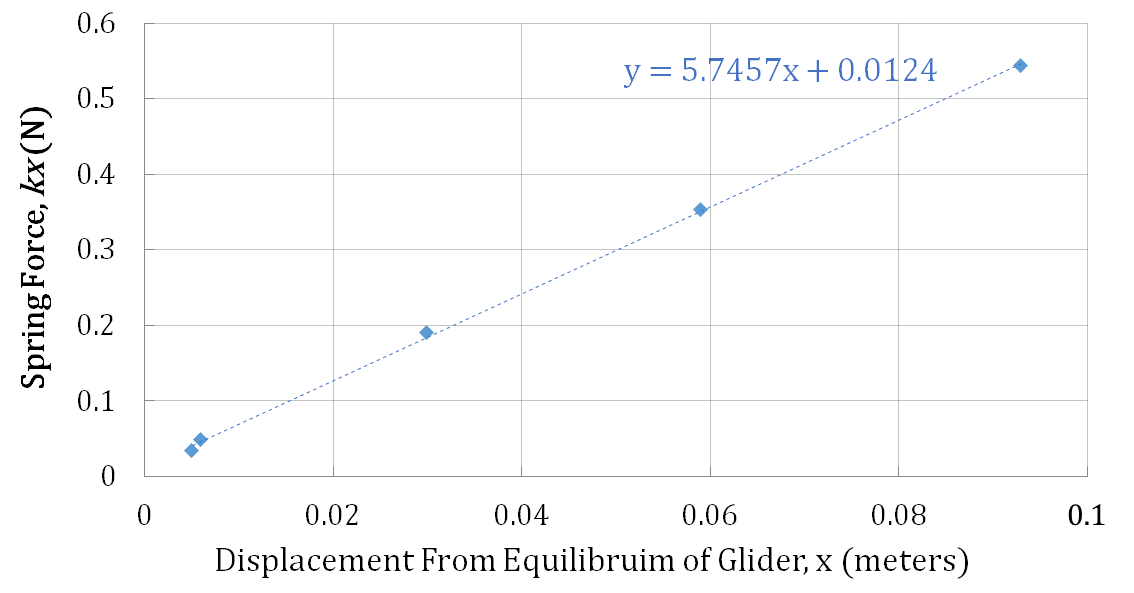
\includegraphics[width=5.0in]{SpringForce.png}
    \caption{Calculation for spring constant $k$. Each blue diamond represents the force applied on the spring glider system by a mass and the subsequent displacement from equilibrium of the glider. The dotted blue line is a linear fit to the data, $F(x) = -kx$, with fit parameter of $k = 5.7457$ $\pm$ 0.0785 N/m. The linear fit line is consistent with zero as the uncertainty of $k$ overlaps with the origin. The negative in the equation $F(x) = -kx$ indicates that the spring force is a restoring force; however, as we are calculating for the magnitude of $k$, we drop the negative. The uncertainty was provided by the Regression tool in Microsoft Excel.}
\end{figure}

From this, we can conclude that the spring constant for this particular glider spring system is $k = 5.75$ $\pm$ 0.08 N/m.

\subsection{Total Energy}

Having all the necessary constants and data points, we can then calculate the total mechanical energy of the system by summing the kinetic energy and the spring potential energy at every given point, which is shown in the plot on the following page:

\pagebreak

\begin{figure}[!htbp]
    \centering
    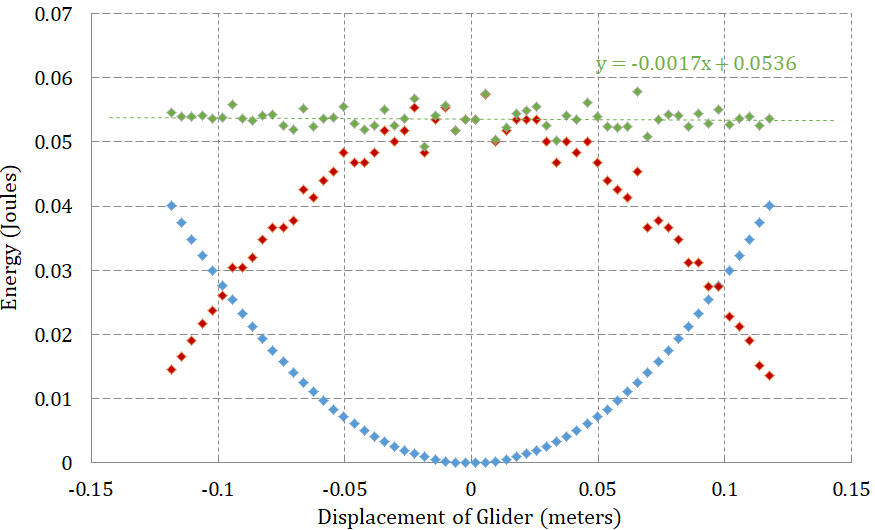
\includegraphics[width=4.75in]{MechEnergy.png}
    \caption{Total energy of the system as a function of displacement. Each blue diamond represents the spring potential energy at the given displacement. Each red diamond represents the kinetic energy of the glider at the given displacement.  Each green diamond represents the total mechanical energy at the given displacement. The dotted green line is a linear fit to the data, $E\textsubscript{total} = -F\textsubscript{friction}x+E\textsubscript{i}$, with fit parameters of $F\textsubscript{friction} = 0.0017$ $\pm$ 0.0030 N and $E\textsubscript{i} = 0.0536$ $\pm$ 0.0002 J. The uncertainty was provided by the Regression tool in Microsoft Excel. Note the increased noise in the kinetic energy of the glider, which is expected when differentiating data.}
\end{figure}

From Figure 3 we can see that while the total mechanical energy remains nearly constant, it does decrease with increased displacement due to the force of friction.

\subsection{Solving for $\mu\textsubscript{k}$}
While there is energy loss due to friction in sources other than just between the air track and the glider, such as air resistance, by assuming the entirety of the loss of mechanical energy to be due to kinetic friction between the air track and the glider, we can use the following equation:

\begin{align}
W\textsubscript{NC} = Fd\cos\theta
\end{align}

The total displacement of the glider over the course of a single measured oscillation (half a period) is two times the amplitude of displacement; in this case, the total displacement is 0.236 meters. Using Equation 2 and the slope of the best fit line from above, we find work not conserved due to friction to be 0.0004 J.

Therefore, the $F\textsubscript{friction}$ = 0.0017 N. Using then the known relationship that $F\textsubscript{friction} = \mu_k F_N = \mu_k mg$, we can solve for $\mu_k$, the coefficient of kinetic friction. Plugging in the mass of the glider and comb, (0.225 $\pm$ 0.001) kg, we find that $\mu_k = 0.0007$. However, this value is incomplete as it lacks the uncertainty.

\subsubsection{Solving for Uncertainty of $\mu\textsubscript{k}$}
Using Equation ii.14 from the lab manual, we can calculate the uncertainty of the coefficient of friction, with $x$ referring to the weight of the glider and comb ($F_N$) and $y$ referring to the value of the slope from the linear fit line ($F\textsubscript{friction}$).

\begin{align}
f &= \mu_k = \frac{F\textsubscript{friction}}{F_N} \\
\delta \mu_k &= \sqrt{\bigg (\frac{\partial f}{\partial x} \delta x\bigg )^2 + \bigg (\frac{\partial f}{\partial y} \delta y\bigg )^2} 
\end{align}

Using the above equations, we find that $\delta \mu_k = 0.001$. Therefore, the final value for the coefficient of kinetic friction is $\mu_k = 0.0007$ $\pm$ 0.0010. This final answer is expected, as the air track is designed to minimize friction and thereby minimize loss of mechanical energy. In the calculation of uncertainty of $\mu_k$, it was found that the mass had a minimal impact on the final uncertainty value. The high value of uncertainty in comparison to the calculated value of $\mu_k$ can be attributed to the fact that the differentiated values for $K$ had a significant amount of noise that was also reflected in the total mechanical energy linear fit equation.

\pagebreak

\section{Conclusion}
From our calculations, we find that the total mechanical energy of the system remains relatively constant, decreasing only slightly due to a comparatively small force of friction, thanks to the low coefficient of kinetic friction between the glider and the air track.

In this experiment, a key contributor to systematic uncertainty is the fact that the maximum amplitude of the glider did not reflect the length of the comb, meaning that we were unable to position the starting position of the glider so that the first tooth was just outside of the photogate. We were unable to do so as if we did position the glider as such, the photogate would not be able to record all 61 teeth as the glider's amplitude of oscillation would be smaller than half the length of the photogate comb.

Consequently, as we positioned the glider farther out than the first tooth, the system began with potential energy that was higher than what was recorded. This in turn means that the potential energy will never equate the total mechanical energy and that the maximum kinetic energy will have a larger magnitude than the maximum potential energy. This in turn leads to increased uncertainty of the total mechanical energy as the system at the moment whereby data begins to be recorded already has kinetic energy. As friction applies on the system throughout, this will in turn cause a higher estimated initial potential (and total) energy.

Further sources of uncertainties and inaccuracies arise from factors such as air resistance, potential initial kinetic energy from an unintended starting ``push'', and the potential fact that the track is not necessarily level, adding in the third factor of gravitational potential energy.

\pagebreak

\begin{thebibliography}{1}
\bibitem{a}
Campbell, W. C. \textit{et al}. Physics 4AL: Mechanics Lab Manual (ver. April 3, 2017).
(Univ. California Los Angeles, Los Angeles, California).
\end{thebibliography}

\end{document}
